% =====================================================================
%  Introduction à la thermique du bâtiment pour les architectes
%  Projet principal : ne contient que la structure du livre.
%  Le contenu est dans le dossier parties/ (un fichier par partie).
% =====================================================================
\documentclass[11pt,a4paper]{book}
% =====================================================================
%  Préambule : packages et réglages communs.
%  Restez sur des packages courants : ceux-ci sont tous compris
%  par la version web du cours.
% =====================================================================
\usepackage[utf8]{inputenc}
\usepackage[T1]{fontenc}
\usepackage[french]{babel}
\usepackage{lmodern}
\usepackage[margin=2.5cm]{geometry}
\usepackage{amsmath,amssymb,amsthm}
\usepackage{graphicx}
\usepackage[hidelinks]{hyperref}

% Numérotation des équations et figures par chapitre : (1.1), (1.2)…
\numberwithin{equation}{chapter}

% Exercices et corrigés
% Sur le site, « exercice » devient un encadré et « corrige » un encadré dépliable.
\theoremstyle{definition}
\newtheorem{exercice}{Exercice}[chapter]
\newtheorem*{corrige}{Corrigé}

% Vos macros
\newcommand{\unite}[1]{\,\mathrm{#1}}


\title{Introduction à la thermique du bâtiment pour les architectes}
\author{Victor De Bono}
\date{ENSAP Lille -- A321 Ambiances}

\begin{document}

\frontmatter
\maketitle

\mainmatter
% =====================================================================
\part{Présentation}
% =====================================================================

\chapter{Introduction}
\label{chap:introduction}

Ce document est le support de cours de l'enseignement A321 Ambiances, dispensé à l'ENSAP Lille. Il ne se substitue pas au cours : il en est plutôt un résumé synthétique.

Ce document est en cours d'élaboration et n'est pas encore finalisé : il peut donc contenir des erreurs.

\chapter{Objectifs}
\label{chap:objectifs}

\chapter{Historique, concepts et unités}
\label{chap:concepts}

\section{Énergie}

\section{Température}

\section{Chaleur}

\section{Propriétés des matériaux}

% =====================================================================
\part{Transferts de chaleur}
% =====================================================================

\chapter{Conduction}
\label{chap:conduction}

\section{Mécanisme de la conduction}

\section{Loi de Fourier}
\label{sec:fourier}

% --- Exemple à conserver ou à remplacer : équation numérotée, renvoi, figure ---
En régime permanent, dans une paroi plane homogène d'épaisseur $e$ et de conductivité thermique $\lambda$, la densité de flux traversant la paroi est proportionnelle à l'écart de température entre ses deux faces :
\begin{equation}
  \varphi = \frac{\lambda}{e}\,(\theta_1 - \theta_2) = \frac{\Delta\theta}{R}
  \label{eq:fourier}
\end{equation}
où $R = e/\lambda$ est la résistance thermique de la couche, en $\mathrm{m^2{\cdot}K/W}$.

Dans chaque couche, la température varie linéairement, avec une pente d'autant plus forte que le matériau est isolant (figure~\ref{fig:profil}).

\begin{figure}[htbp]
  \centering
  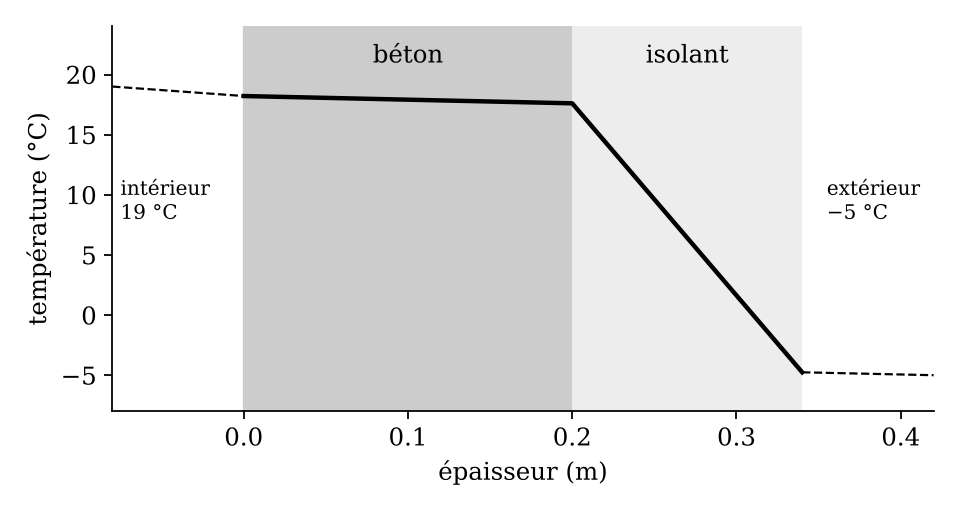
\includegraphics[width=0.7\linewidth]{figures/profil-temperature.png}
  \caption{Profil de température dans un mur en béton isolé par l'extérieur.}
  \label{fig:profil}
\end{figure}
% --- Fin de l'exemple ---

\section{Conduction dans les parois}

\section{Ponts thermiques}

\section{Isolation}

\section{Exercices}

\begin{exercice}
Un mur est composé de 20~cm de béton ($\lambda = 2{,}0\unite{W/(m{\cdot}K)}$) et de 14~cm de laine de bois ($\lambda = 0{,}038\unite{W/(m{\cdot}K)}$). Calculer la résistance thermique de chaque couche à l'aide de l'équation~\eqref{eq:fourier}.
\end{exercice}

\begin{corrige}
Béton : $R = 0{,}20 / 2{,}0 = 0{,}10\unite{m^2{\cdot}K/W}$. Laine de bois : $R = 0{,}14 / 0{,}038 \approx 3{,}68\unite{m^2{\cdot}K/W}$.
\end{corrige}

\chapter{Convection}
\label{chap:convection}

\section{Mécanisme de la convection}

\section{Convection naturelle et convection forcée}

\section{Convection dans le bâtiment}

\chapter{Rayonnement}
\label{chap:rayonnement}

\section{Mécanisme du rayonnement}

\subsection{Le Soleil}

\subsection{Les ondes électromagnétiques}

\section{Apports solaires}

\section{Rayonnement dans le bâtiment}

\chapter{Conclusion sur les transferts de chaleur}

% =====================================================================
\part{Transferts de vapeur}
% =====================================================================

\chapter{Passage de la vapeur}
\label{chap:vapeur}

\section{Pression de vapeur et humidité}

\section{Transfert de vapeur}

\section{Diagramme de l'air humide}

\section{Vapeur dans le bâtiment}

\chapter{Pression de vapeur dans une paroi}

\chapter{Conclusion sur les transferts de vapeur}

% =====================================================================
\part{Climat}
% =====================================================================

\chapter{Effet de serre}

\chapter{L'ère de l'Anthropocène}

\chapter{Dérèglement climatique}

\chapter{Conclusion sur le climat}

% =====================================================================
\part{Thermique architecturale}
% =====================================================================

\chapter{Régime dynamique}

\chapter{Enveloppe}

\chapter{Confort}

\section{Confort d'hiver}

\section{Confort d'été}

\chapter{Équipements}

\section{Ventilation mécanique contrôlée (VMC)}

\section{Chauffage}

\section{Climatisation}

\chapter{Conclusion sur la thermique architecturale}

% =====================================================================
\part{Cadre réglementaire}
% =====================================================================

\chapter{RT 2012}

\chapter{Expérimentation E+C$-$}

\chapter{RE 2020}

\section{Carbone}

\section{Énergie}

\section{Confort d'été}

\chapter{Conclusion sur le cadre réglementaire}

% =====================================================================
\part{Conclusion et perspectives}
% =====================================================================

\chapter{Synthèse}

\chapter{Interventions}

\section{Projet neuf}

\section{Projet de réhabilitation}

\chapter{Pour aller plus loin}


\end{document}
